\documentclass[11pt,a4paper]{ivoa}
\input tthdefs

\usepackage{array}
\usepackage{tabulary}  % for nicer tables
\usepackage{calc}
\usepackage{placeins}
\setlength\extrarowheight{2pt}

\newcolumntype{L}{>{\centering\arraybackslash}m{3cm}}
\title{MANGO: A Component and Association Based Model for representing data for astronomical sources}

% see ivoatexDoc for what group names to use here
\ivoagroup{DM}


% mireille commands
% borrowed from Prov WD - Kristin - own definitions
\definecolor{todocolor}{rgb}{1,1,0.8}
\definecolor{darkred}{rgb}{0.6,0,0}
\definecolor{rose}{rgb}{1.0,0.88,0.88}
\definecolor{darkgrey}{rgb}{0.35,0.35,0.35}
%\newcommand{\TODO}[1]{%
%    \noindent%
%    \textcolor{todocolor}{\sffamily [\textbf{TODO:} #1]}%
%}

\newcommand{\TODO}[1]{%
    \noindent%
    \colorbox{todocolor}{%
            \parbox{0.85\linewidth}{\sffamily \textbf{TODO:}\\
            #1}
    }%
    \vspace{2pt}

}

\newcommand{\note}[1]{%
    \noindent%
    \textcolor{darkgrey}{{\sffamily Note:} \emph{#1}}%
}

\newcommand{\comment}[1]{%
    \noindent%
    \textcolor{red}{{\sffamily Comment:} \emph{#1}}%
}
% end mir commands


\author{François Bonnarel}
\author{Gilles Landais}
\author{Laurent Michel}
\author{Jesus Salgado}
\author{Mireille Louys}
\author{Marco Molinaro}

\editor{Laurent Michel}

% \previousversion[????URL????]{????Concise Document Label????}
\previousversion{This is the first public release}

\begin{document}
\begin{abstract}
The MANGO model proposes a flexible way to expose data related to astronomical source objects in an interoperable way.
It takes into account the huge diversity of source data in terms of feature description, format and usage.
The MANGO model attaches identifiers on astronomical sources and associates to each a flexible set of parameters (e.g. observed physical quantities) and other information like e.g. spectra, time series or preview images.
Parameters usually appear in the columns of a source catalogue. Additional data products are bound to the source to contribute to the science analysis and enhance data understanding.
Mango object parameters are built upon classes or extended classes of the IVOA Measure and Coordinates data model.
Associated data can be simple URLs, VO service endpoints or VO data model instances.
The roles of both parameters and associated data are qualified by semantic tags

\end{abstract}


\section*{Acknowledgments}

We would like to thank all those who took the time to present their own use cases (INAF, CDS, CFA, ESAC) on which the model has been built.
We would also like to thank all the people having tested MANGO on their own data.

\section*{Model Name}
This model was initially named with a very explicit but hard to remember acronym, \texttt{CAB-MSD} standing for Component and Association Based Model for Source Data. We decided later to rename it \texttt{MANGO} with reference to the inside out MANGO picture used to introduce the model in Groningen. As the tradition requires that such unexpected names are acronyms, let's assume that \texttt{MANGO} stands for
%mir Model Adding Necessaries to Generic Objects.
Metadata ANnotation for Generic Objects (in astronomy).


\section*{Conformance-related definitions}

The words ``MUST'', ``SHALL'', ``SHOULD'', ``MAY'', ``RECOMMENDED'', and
``OPTIONAL'' (in upper or lower case) used in this document are to be
interpreted as described in IETF standard RFC2119 \citep{std:RFC2119}.

The \emph{Virtual Observatory (VO)} is a
general term for a collection of federated resources that can be used
to conduct astronomical research, education, and outreach.
The \href{http://www.ivoa.net}{International
Virtual Observatory Alliance (IVOA)} is a global
collaboration of separately funded projects to develop standards and
infrastructure that enable VO applications.


\section{Introduction}

Modeling data collected to study astronomical source objects has been a long term concern for the DM working group and more generally for the IVOA.
In the past years, there were some proposals to design a global model for sources \citep{wd:jesusdm} as well as for catalogs \citep{wd:catalog}.
Other proposals, more model-agnostic, were focused on the data annotation in VOTables \citep{note:stcvot} \citep{note:seb}. 
In this case the goal was no longer to design a source model but to provide a complete description of  individual quantities (positions, velocity, fluxes, magnitudes…).
None of these proposals have come to completion.

The source DM issue resurfaced at the spring 2018 Interop in Victoria during an hands-on session focusing on the tools available to work with VO data models and especially with VO-DML. 
The goal of this session was to annotate data from different origins in order to make them interoperable with each other.
%mir The main concern expressed during this session was not much related to the tools themselves but indeed to the lack of models for sources.
One of the main concerns outside de tools necessary to workout this notation was the lack of models for source objects.
This is a big paradox in the VO world: source data which represent the basic building blocks of astronomers' work, is not modeled. 
This paradox can be explained by the fact that the observation of source objects is multi-faceted.
In a general way, the way features for source data are described and organized depends on the targeted science case. 
Principal investigators and archive designers set up the data profile and structure it according to this goal which varies from one project to another. 
Therefore this diversity cannot be served by a single static data model describing a source item for all possible cases.
Having a global source model would lead to a very complex solution not usable in practice.

This standard proposes to overcome this paradox and presents a template model gathering independent components from VO existings models 
together with VO data products and files embedded on demand in a container.
The template supports fine grain association by composing classes as well as coarse grain relations to data products and files distributed within projects archive.
Mango is not designed to describe what a source is but to help clients to discover and to understand the quantities available for a particular source instance.

\subsection{Role within the VO Architecture}

\begin{figure}
\centering

% As of ivoatex 1.2, the architecture diagram is generated by ivoatex in
% SVG; copy ivoatex/archdiag-full.xml to archdiag.xml and throw out
% all lines not relevant to your standard.
% Notes don't generally need this.  If you don't copy archdiag.xml,
% you must remove archdiag.svg from FIGURES in the Makefile.

\includegraphics[width=0.9\textwidth]{role_diagram.pdf}
\caption{Architecture diagram for this document}
\label{fig:archdiag}
\end{figure}

Fig.~\ref{fig:archdiag} shows the role this document plays within the
IVOA architecture \citep{note:VOARCH}.



\section{Representing observed astronomical objects : Use Cases and  Requirements}

\subsection{Use Cases}
The following uses-cases have been collected since 2019 from representatives of various astronomical missions, archive designers and tools developers.
The contribution was totally open. This gave a good picture of the needs but we don not pretend that everything will be supported by this first version.

%\TODO{ may be too early to conclude about this ?? The contribution was totally open. 
%This gave a good picture of the needs but it's safe to say that not everything will supported by this first version.??}

The physical parameters recorded for each source in the various projects are listed below:
\subsubsection{Gaia}
\begin{itemize}
    \item identifier
    \item sky reference position
    \item proper motion
    \item parallax and distance

    \item source extension
    \item radial velocity
    \item redshift
    \item photometry
    \item date of observation ?
    \item correlation ( with other sources ?)
    \item multiple detection
\end{itemize}


\subsubsection{Euclid}
\begin{itemize}
    \item identifier
    \item sky position
    \item correlation with Gaia counterpart?
    \item photometry (ground + satellite )
    \item morphology class?
    \item redshift
    \item photometric redshift
\end{itemize}

\subsubsection{Exoplanets missions}

\begin{itemize}
    \item position
    \item orbit
    \item different source level (source types instead?)(star, planet, moon)
    \item status and classification
    \item orbiting system description
\end{itemize}

\TODO{mention the involved projects : examples ? GAPS, TESS? }
\subsubsection{Morphologically Complex Structures}

\begin{itemize}
    \item morphology
\end{itemize}

\TODO{to be developed ...}

\subsubsection{Chandra Archive}
This X-ray mission has produced a very large catalog of sources. %( ?? TB) \cite{chandra catalog, 2019}. https://cxc.harvard.edu/csc/organization.html
All quantities are time dependant, depend on calibration methods as well as on appropriate physical
models that selects energy models for the origin of the recorded photons ...


\TODO{to be developed, explained ...}
\begin{itemize}
    \item name
    \item pos
    \item time
    \item extension
    \item PHA ???
\end{itemize}

\subsubsection{Vizier catalog archive  }

% GILLLES proposal:
%
VizieR provides science ready catalogues coming from space agencies or articles and covering number of different science cases. 
Published data encompass a very large set of measures (position, photometry, redshift, source type, etc.) depending on their origin. 
They can result from  observations, simulations, models or catalog compilations.
Individual Vizier tables can contain data all related to one source (e.g. time series of positions or magnitudes) or to a set of sources (one row per source) or a mix of both.  
%The most frequent are observation tables which can serialize a single object to one or more records.
%
Data sets are ingested in Vizier on author request. Before to be put online they are processed and documented by documentalists so as to ensure a certain level of interoperability.
This work relies on the analyse of both data content and scientific paper.
\begin{itemize}
\item Missing meta-data, e.g. space frames or filters, are added when available in the paper.
\item Columns are renamed following the Vizier nomenclature in order make them compliant with the DBMS and to facilitate the grouping of all values related to one particular quantities (e.g. quality flag for a radial velocity)
\item UCDs are checked or set for all columns.
\item README files are generated. A README is a text file with a specific layout making it machine readable.
\item Some values, not part of the original data but assigned by the CDS, are added to the tables (e.g. identifier, ICRS positions)  
\item Ancillary data pointing on associated data (e.g.  spectra) or on linked services (e.g. visualization), can also be added to enrich the table content.  
\end{itemize}

All Vizier meta data are gathered in a specific resource in a way to facilitate the localisation of data of interest.
The main specificity of the data is their heterogeneity 
\begin{itemize}
\item Huge variety of data provenance and processing 
\item Meta data heterogneneity
\item Table content heterogneneity
\item Huge variety of possible measures
\item Huge variety of patterns of measure groups
\item Use of different coodinate systems 
\item Large variety of associated data
\end{itemize}

The Mango model must be able to provide a standard representation of most of the metadata contained in Vizier query responses, whether native or computed  by the CDS, simple quantities or associated complex data.
Mango is not meant to replace the current management of the meta-data, it is a way to make those meta-data understandable for a wide panel of VO-compliant clients.

%The tables processed are documented and standardized in order to be interoperable. The metadata includes coordinates systems  and  the magnitudes columns can be completed with photometric paremeters –these last metadata are not part of the original data but are assigned by CDS.
%
%The records can also be competed with added columns like links to local or remote URL, visualization of time-series,  etc.
%
%The table output allows for anyone aware of the VizieR nomenclature to group columns related to a given measure. 
%
% The VizieR tables can be charcterized by :
%\begin{itemize}
%\item the heterogneneity of the table contents
%\item a large variety of possible measure that can be grouped by type
%\item different coodinate system 
%\item different metadata processing and provenance
%\item different object serialization 
%\item added-data sometimes available for objects records
%\end{itemize}
%
% END GILLLES proposal


Vizier gathers and delivers a curated version of published catalogs from various missions and experiments.
It also distributes results of scientific papers, based on the computation , comparison and classification of sources extracted from archived data after science analysis.
Vizier handles a very large set of measures in position, photometry, redshift, source type, etc.
% FB : I don't think the end of this sentences was correct : "as authors original data."
It adds value to it by recomputing additional quantities in various reference frames or equivalent spectral bands, units conversions , etc .
It binds the resulting object description to other data sets representing the object, or its counterparts, or neighbourhood on sky (image), its spectral behaviour (spectrum, spectral energy distribution) or evolution through time (light curve, radial velocity curve, timeseries, etc.).
Currently the binding and structure of the quantities is done by column grouping.
\begin{itemize}
    \item pre-existing data
    \item grouping columns
    \item lots of available metadata
    \item column name formatting
    \item one column different frames
\end{itemize}

\subsubsection{Client on (MT behalf)}

Right now, the meta-data provided within the VOTable allow clients such Aladin or Topcat to run most of the functionalities expected by the user, either for data analysis of plotting.
This information is often guess from UCDs, UTypes or columns name. It can aloso be given by the user.
Clients have no expectations of working with full model instances but in some cases models can help to know how quantities in an input table relate to each other.
In most cases this is for visualisation, e.g.:
\begin{itemize}
    \item what is the sky position for this row
    (what columns contain lat and lon, and what sky system are they in)

     \item what +/-ERR error bars should I plot for these points
    (what column is a simple error for column A)

    \item what error ellipses should I plot for these sky positions
    (what columns provide ra\_error, dec\_error, ra\_dec\_corr,
     or how can I derive those from columns that do exist)

    \item where do I get the grid information for a column containing
    a vector of samples so I can label the X axis of a spectrogram
    (what column or parameter contains an axis vector matching
     the sample vectors)

    \item does this table contain sky positions, or HEALPix tiles, or both?
    What's the best way to represent it on the sky?
    
    \item What is the meaning of such URL found out in a table?s
\end{itemize}

But there are some other places too:
\begin{itemize}
    \item how do I propagate this sky position to a future epoch
    (what columns contain pmra, pmdec, and maybe all the
     associated errors and correlation coefficients)

    \item what is the error ellipse/oid to use for a sky/Cartesian crossmatch
    (what columns provide the relevant errors and, if available,
     correlations)
\end{itemize}

This usage shows that MANGO must be designed in a way that individual measurements or quantities can be easily be identified as such and manipulated independently of the whole instance.


\subsubsection{Xmatch tool }

The basic cross-match of two astronomical tables consists in associating pairs of sources -- one from each table -- fulfilling a given angular distance based criterion.
In relational algebra terms, it is a theta-join on a distance predicate.

More generally, a cross-match is the association of sources from different tables given their proximity in an astrometrical (but also possibly photometric, statistical, ...) parameter space \citep{2017A&A...597A..89P} .

If proper motions (plus parallax and radial velocities) are available, the cross-match tool may propagate the positions of each table to a common epoch.
It may also take into account positional uncertainties to reject the statistically unlikely associations.

In the latter case (cross-match between two tables taking into account positional errors), the tool needs to be able to retrieve the errors associated to the each position in each table.

UCDs may help in identifying the errors associated to a positional columns as shown in table \ref{tbl::pos-errors}.


\begin{table}[!htbp]
\small
\centering
\begin{tabulary}{\linewidth}{|L|C|J|}
       \hline
           \textbf{Error type  \newline Parameters} &  
           \textbf{UCD} &        
           \textbf{Description} \\
       \hline 
           \multicolumn{3}{c}{\textbf{Circular error}} \\
       \hline
           \texttt{epos}&

           \texttt{stat.error;pos.eq}    & 
           See "possible ambiguity for circular errors" \\     
        \hline  
           \multicolumn{3}{c}{\textbf{Uncorrelated errors}} \\
        \hline
           \texttt{eRA}     &            
           \texttt{stat.error;pos.eq.ra}    & 
            Error on `RA cos(Dec)` \\              
         \hline
            \texttt{eDec}  &
           \texttt{stat.error;pos.eq.dec}    & 
            Error on `Dec`\\              
         \hline  
            \multicolumn{3}{c}{\textbf{Correlated errors}} \\
        \hline
           \texttt{eRa}  &            
           \texttt{stat.error;pos.eq.ra}    & 
           Error on `RA cos(Dec)` \\              
        \hline
           \texttt{eDec}&
           \texttt{stat.error;pos.eq.dec}   &
           Error on `Dec`     \\              
        \hline
            \texttt{corRADec}&
           \texttt{stat.covariance; pos.eq.ra; pos.eq.dec }    & 
            Correlation factor\\              
        \hline
             \multicolumn{3}{c}{\textbf{Oriented Ellipse}} \\
        \hline
           \texttt{a}   &            
           \texttt{phys.angSize.smajAxis; pos.errorEllipse}    & 
           Error ellipse semi-major axis \\              
        \hline
            \texttt{b} &
           \texttt{phys.angSize.sminAxis; pos.errorEllipse }    & 
            Error ellipse semi-minor axis \\              
        \hline
            \texttt{theta}  &
           \texttt{pos.posAng; pos.errorEllipse}    & 
           Error ellipse position angle \\              
       \hline 
\end{tabulary}
\caption{Table of the different possible representations of positional errors that can be found in astronomical catalogues} 
\label{tbl::pos-errors}
\end{table}

But this is not sufficient to takle with more complex cases based on multi-parameter cases: 

\begin{itemize}
	\item Catalogues like AllWISE provides a co-sigma instead of the correlation factor of the covariance matrix.
	Co-sigma is the sign of the correlation factor time the square root of the covariance.
	\item Table fields UCDs  may be too loose: for example  \texttt{stat.error;pos.eq} is often used in place of \texttt{phys.angSize.smajAxis;pos.errorEllipse} or \texttt{phys.angSize.sminAxis;pos.errorEllipse}.
	\item The location  of the column to be used for the Xmatch can be ambigous. For instance, if several pairs of position are provided in a table, there is currently 
	no way to associate unambiguously uncertainties with the (right) pair of coordinates.
	\item  Possible ambiguity for circular errors. When the provided uncertainty is the parameter of a circular error, it may be:
	\begin{itemize}
		\item either the 1 dimensional component on each axis of a symmetric 2-dimentional Gaussian distribution: $\sigma=\sigma_{\alpha\cos\delta}=\sigma_\delta$;
		\item or the parameter of the radial error distribution (i.e. of the Rayleigh distribution): $\sigma=\sqrt{\sigma_{\alpha\cos\delta}^2 + \sigma_\delta^2}$
                 with $\sigma_{\alpha\cos\delta} = \sigma_\delta$
         \end{itemize}

	\item   Possible ambiguity on the confidence level
	The provided error is usually the 1sigma error.
	It (theoretically) means that the "true" position has:
	\begin{itemize}	
		\item either 68\% chances to be at a distance lower than the radial error from the position's mean value.
		\item or 39\% chances to be inside the error ellipse (or circle) around the position's mean value.
	\end{itemize}
	But depending on the catalogue, the provided error parameters can correspond todifferent confidence levels.

\end{itemize}


\subsection{Requirements}

\subsubsection{Parameters and Associated Data}
From the use-cases' description, two categories of features must provided or foreseen by the projects:

  \begin{itemize}
    \item The source \emph{parameters} astronomers will investigate for their science. They are measures provided as numerical values or classification tags exposed as numbers or simple strings. Usually on measure corresponds to one individual column or one group of columns .
     \item The \emph{Associated data} are generally science ready dataproducts either from the same project, or shared by other projects within the IVOA interoperability framework.
They bring a complement of information to interpret the source's  parameters under study and compare visually (or computationnaly) the sky neighbourhood of detected sources, their variation through time or spectral behaviour.
Referencing such datasets by a URI or by a service endpoint already works for existing VO products. ( It has been promoted and recommended in Obscore / Spectrum Dm, . etc for access URIs, and DataLink for service endpoints REFS).
Associated data can also present a complex structure designed to bring a very advanced context of interpretation (CTA model assumptions, energy model for Xray sources, etc. REFS) which need to be described in the attachement.
 \end{itemize}     
  %   They are usually described in astronomical catalogs by columns description in a table. 
 % \end{itemize}
%  , the results from the analysis of the observed or simulated data for sources on one side, expressed as physical measures and classification results like types, status, etc. and extra information provided for interpretation purpose on the other side and expressed as % % %%\emph{associated data}.
%Features in each project are measures provided as numerical values or classification tags exposed as numbers or simple strings. They are the source \emph{parameters} astronomers will investigate for their science.
%They are usually described in astronomical catalogs by columns description in a table. The source instances recorded by the projects feed the rows of such tables.
%VOTable has been till today the format of choice to distribute such data.

% mir trop tot ds la partie uses-cases --> partie model ? The MANGO datamodel describes measures by relying on the IVOA Meas data model.%\cite{MEAS}.
%Associated data are generally science ready dataproducts either from the same project, or shared by other projects within the IVOA interoperability framework.
%They bring a complement of information to interpret the source's  parameters under study and compare visually (or computationnaly) the sky neighbourhood of detected sources, their variation through time or spectral behaviour.
%Referencing such datasets by a URI or by a service endpoint already works for existing VO products. ( It has been promoted and recommended in Obscore / Spectrum Dm, . etc for access URIs, and DataLink for service endpoints).
%Associated data can also present a complex structure designed to bring a very advanced context of interpretation (CTA model assumptions, energy model for Xray sources, etc.) which need to be described in the attachement.

%Table  \ref{tab:q_breakup} summarizes the features and related quantities exposed in the various use-cases. The two categories clearly show up.



%\begin{table}[ht!]
  %   \tiny
 %    \begin{tabular}{|p{2.4cm}|p{0.4cm}|p{0.4cm}|p{0.4cm}|p{0.6cm}|p{0.4cm}|p{0.4cm}|p{0.4cm}|p{0.4cm}|p{0.4cm}|}
%       \hline Quantity/ Survey &  Ga &  Eu &  Ex &  MCS  &  Ch&  Vi &  Al &  Xm&  TD \\
%       \hline  \texttt{identifier}      &  p & P  &P& &P&P &P&  & P \\
%       \hline  \texttt{position}      &  p & P  &P& &P&P &P&  & P \\
%       \hline  \texttt{pr. motion}   & p &   &   &    &  &   &P&P&    \\
%       \hline  \texttt{distance}     & p &   &   &    &  &   &P&  &    \\
%       \hline  \texttt{correlation}   & AD &AD&   &    &  &AD &   &  &    \\
%       \hline  \texttt{extension}     &P&   &P&P &P&P& P&  &    \\
 %      \hline  \texttt{rad. vel.}       &  P &   &   &    &  &P&   &  &    \\
%       \hline  \texttt{redshift}        &  P &P&   &    &  &P&   &  &    \\
 %      \hline  \texttt{phot. rsft}      &   &P&   &    &  &P&   &  &    \\
 %      \hline  \texttt{luminosity}    & P&P&   &    &  &P&P&P&P\\
 %      \hline  \texttt{date}             & P  &   &   &    & P&P&   &  &P\\
 %      \hline  \texttt{detections}    &  AD &   &   &    &  &   &   &  &    \\
  %     \hline  \texttt{orbit}             &   &   &P& &  &   &   &  &    \\
 %      \hline  \texttt{type}             &   &   & P& &  &P&   &  &    \\
 %      \hline  \texttt{status}          &   &   &   &    &  &P&   &  &    \\
 %      \hline  \texttt{orb. sys.}      &   &   &  P &    &  &   &   &  &    \\
  %     \hline  \texttt{PHA}            &   &   &   &    &P&   &   &  &    \\
 %      \hline  \texttt{assoc. products}     &   &   &   &    &  &AD&   &  &AD \\
 %      \hline
 %    \end{tabular}
 %    \caption{ Break up of the requested quantities:  \texttt{P} stands for Parameter, \texttt{AD} for Associated Data}

 %    \label{tab:q_breakup}
% \end{table}

\subsubsection{R01: Supported Quantities}
\begin{itemize}
    \item MANGO must provide unique source identifiers.
    \item MANGO must provide modeling classes for both parameters and associated data.
    \item The number of parameters attached to a MANGO instance must be free.
    \item The number of associated data attached to a MANGO instance must be free.
\end{itemize}

\subsubsection{R02: Parameters}
The concept of \texttt{Parameter} matches the concept of measure of the Meas model. MANGO may support Parameter classes that are not Meas classes though.


\begin{itemize}
    \item MANGO must support explicit classes imported from an IVOA datamodel for the most used parameters.
    \item MANGO must provide a generic way to support parameters that do not enter the above category.
    \item MANGO instances must support multiple instances of the same parameter class.
    \item The presence of any parameter in MANGO instances must be optional.
    \item MANGO must provide a way to identify the role of each parameter.
     \item  MANGO must provide a way to describe the meaning of flags or qualifiers.
    \item The role of each parameter should be machine-readable.
    \item It must be possible to group parameters in a free way. This allows to tag quantities with timestamps or a flags. 
\end{itemize}

\subsubsection{R03: Associated Data}
The notion of associated data relates to any sort of complex data. This can be a pointer to a service or a data set, a data table or  other data structure.
\begin{itemize}
    \item MANGO must support references to external datasets.
    \item MANGO must support references to external services.
    \item MANGO must support references to other MANGO instances.
    \item MANGO  must support references to instances of models serialized in VO-DML.
    \item MANGO instances must support multiple instances of the same associated data class.
    \item The presence of any associated data in MANGO instances must be optional.
    \item MANGO must provide a way to identify the role of each associated data in order to explain which purpose is served when associating this data to the source object.
    \item The role of each associated data should be machine-readable.
 \end{itemize}

\section{Model Overview}

\begin{figure}
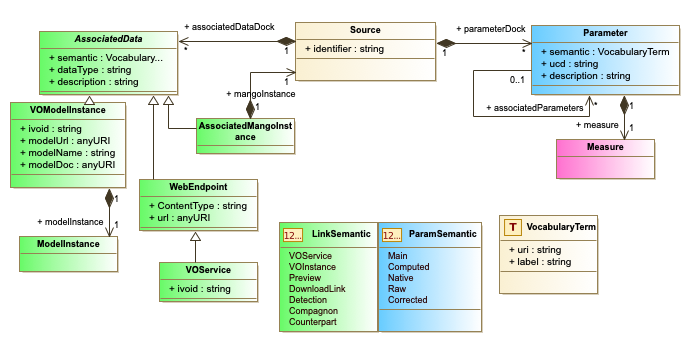
\includegraphics[width=0.9\textwidth]{../model/mangoOverview.png}
\caption{MANGO overview}
\label{fig:overview}
\end{figure}


Sky objects are represented by instances of the class \texttt{MangoObject} which has only one mandatory attribute, the source \texttt{identifier}.
It is recommended the identifiers to be unique within a source collection e.g. a catalog.

The \texttt{MangoObject} is a dock for all source parameters and for all data associated to that source.
The pattern of either parameters or associated data attached to a source is not specified by the model. It depends of the data set on which the model is applied.

The \texttt{MangoObject} has one connector for the paremeters,  the \texttt{parameters} relation, and another for the associatedData, the  \texttt{associatedData}  relations.
Both connectors have an open-ended cardinality.

Each source paremeter is hooked to the \texttt{MangoObject} by a wrapping class (\texttt{Parameter} ) that contains anything necessary to identify its nature and roler.
Parameters can be linked together to represent logical parameter sets. These logical sets have no semantic. Their interpretation is in charge  of the clients.

Each associated data or data pointer is hooked to the \texttt{MangoObject} by a wrapping class (\texttt{AssociatedData}) that contains anything necessary to identify its nature and its role.

\subsection{Parameters}

\texttt{Parameter}  connectors are used to bind measures with the source.
A parameters is composed  by semantic tags in addition to the measure itself, instance of \texttt{Measure}.

 \texttt{Measure} is an abstract class imported from \texttt{meas} model. 
Concrete classes referended by a \texttt{Parameter} instances are either \texttt{meas}  built-in classes or  \texttt{Measure} sub-classes being part of Mango.

\subsubsection{Parameters Identification}
As the parameter set  attached to a particular instance is not defined by Mango, the model must provide an accurate parameter description to allow the client to figure out what it can do with each of them.
Mango provides 5 description levels for each parameter:

\begin{itemize}
    \item \textbf{Measure class (vodml type)}: measures are modeled by specific  \texttt{Measure} sub-classes.
              Knowing that class tells the clients  how to interpret the corresponding measure but does not help much to get its role e.g. a position can be either a source postion or a pointing direction.
              Furthermore, unusual measures e.g. magnetic field,  are represented by  \texttt{GenericMeasure} . 
              In that case, the vodml type does not help at all.
    \item \textbf{UCD}: A valid UCD must be attached to each parameter. 
              Mango provides a UCD space for each \texttt{Measure} sub-class . 
              UCDs used for specific measures must be compliant with table \ref{tab:ucds}. 
              For generic measures, the UCD choice is in charge of the data provider. 
              In any cases, the consistance between UCDs and measure is the responsability of the data provider.
 
    \item \textbf{Reduction status (model enumeration)}: A reduction level of the parameter (e.g. a parameter can be calibrated or not or it can be a computed qualifier) may be attached to the parameter.
    \item \textbf{Semantic}: A reference to  a valid vocabulary word may be attached to each parameter. The choice of that vocabulary is totally free as long as it is published.
    \item \textbf{Description}: A free text description may be attached to each parameter.
 \end{itemize}

\TODO{TBC phys.luminosity  vs phot.flux}
\begin{table}[ht!]
     \begin{tabular}{|p{4.2cm}|p{3cm}|p{3.5cm}|}
       \hline Parameter &  Original model & UCDs 1+ first word  \\
       \hline  \texttt{Position}             &  Measure  &  pos \\
       \hline  \texttt{Velocity  }            &  Measure & phys.veloc      \\
       \hline  \texttt{Proper motion}    & Measure & pos.pm    \\
       \hline  \texttt{Time}                   & Measure &  time.epoch   \\
       \hline  \texttt{Polarization}         & Measure & phys.polarization \\
       \hline  \texttt{LonLatSkyPosition}    &  MANGO  &  pos.eq \\
       \hline  \texttt{Redshift}                        &  MANGO  & src.redshift \\
       \hline  \texttt{Luminosity}                    &  MANGO  & phot.qqqchose \\
       \hline  \texttt{HardnessRatio}             &  MANGO  & phot.flux;arith.ratio \\
       \hline  \texttt{Shape}                     &  MANGO  & phys.area \\
       \hline  \texttt{Flag}                        &  MANGO  & meta.code  \\
       \hline  \texttt{Orbit}                       &  MANGO  & src.orbital \\
       \hline  \texttt{Generic(String)Measure}    &  Measure  &  Appropiate physical UCD \\
       \hline
     \end{tabular}
     \caption{ UCDs soace to be used for the supported parameters}
     \label{tab:ucds}
 \end{table}



\subsubsection{Measure Extension}

All \texttt{Measure} classes are built upon the same pattern (see Fig \ref{fig:stcpattern}). 
\begin{itemize}
  \item  \texttt{Measure} instances are made with an \texttt{Error} and a \texttt{Coordinate} that contains the measure value(s).
   \item  The  \texttt{Coordinate} includes a  \texttt{CoordSys} instance describing the coordinate system relevant for that measure.
   \item The coordinate system has two components : the space  ( \texttt{CoordSpace} class) that describes the axis and the frame (\texttt{CoordFrame} class).  
 \end{itemize}
 
MANGO parameters are all based on this pattern. 
Native  \texttt{Measure} classes are used whenever possible. 
Others Parameters are built by extending this class as shown in figure \ref{fig:stcpattern}). 
These extended classes are part of MANGO.
\begin{figure}
     \includegraphics[width=1.0\textwidth]{stc_pattern.png}
     \caption{Measure/Coordinate pattern (simplified view)}
     \label{fig:stcpattern}
\end{figure}

\begin{figure}
  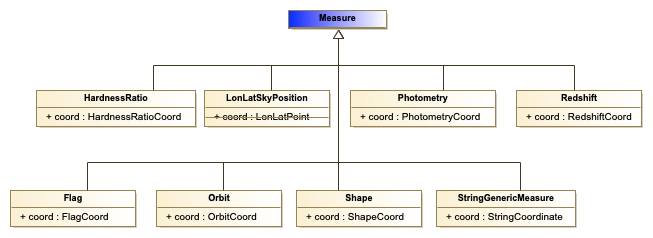
\includegraphics[width=1.0\textwidth]{../model/mangoMeasures.png}
  \caption{Mango extensions of Measure.}
  \label{fig:measures}
\end{figure}

\begin{figure}
  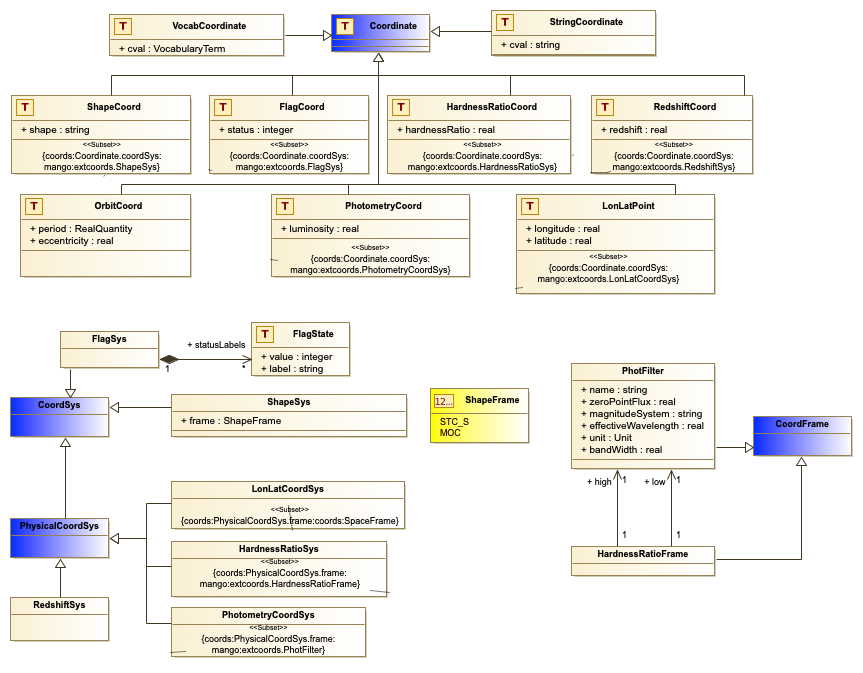
\includegraphics[width=1.0\textwidth]{../model/mangoCoordinates.png}
  \caption{Mango extensions of Coordinates.}
  \label{fig:coordinates}
\end{figure}

\begin{figure}
  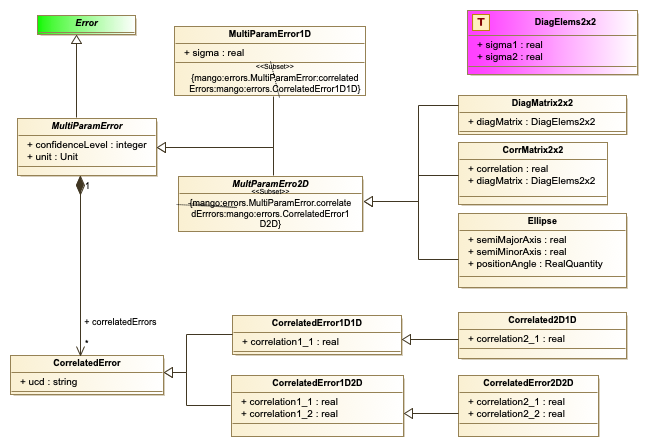
\includegraphics[width=1.0\textwidth]{../model/mangoErrors.png}
  \caption{Mango correlated errors.}
  \label{fig:errors}
\end{figure}



%\begin{table}[ht!]
 %    \tiny
%     \begin{tabular}{|p{2.4cm}|p{1.8cm}|p{7cm}|}
%       \hline Quantity &  Model &  \\
%       \hline  \texttt{identifier}      & MANGO & required for anu instance\\
%       \hline  \texttt{position}      &  Meas &  \\
%       \hline  \texttt{pr. motion}   & Meas &     \\
%       \hline  \texttt{distance}     & Ext Meas &     \\
%       \hline  \texttt{correlation}   & Ass data & reference to other MANGO instances     \\
%       \hline  \texttt{extension}     & Ext Meas & Can be used for FoV, morphlogy or shape\\
%       \hline  \texttt{rad. vel.}       &  Ext Meas  &       \\
 %      \hline  \texttt{redshift}        &   Ext Meas  &  \\
%       \hline  \texttt{phot. rsft}      & Ext Meas&    \\
%       \hline  \texttt{luminosity}    & Ext Meas&\\
 %      \hline  \texttt{date}             & Meas & date or time stamp\\
 %      \hline  \texttt{detections}    & Ass data & reference to other MANGO instances   \\
 %      \hline  \texttt{orbit}             & Ext Meas&      \\
 %      \hline  \texttt{type}             &Ext Meas&     \\
 %      \hline  \texttt{status}          &Ext Meas&     \\
 %      \hline  \texttt{orb. sys.}      &Ext Meas&     \\
 %      \hline  \texttt{PHA}            &Ext Meas&     \\
 %      \hline  \texttt{ass. prd.}     &Ass data&  \\
 %      \hline
%     \end{tabular}
 %    \caption{ Mango quantities with  corresponding complex type  \texttt{Native Meas} Measure class, \texttt{Ext Meas } Measure extension, \texttt{Ass data  } Mango associated data}
% \end{table}



\subsection{Associated Data}

\texttt{AssociatedData} connectors are used to bind any sort of complex data with the source.
One connector can only refer to one dataset.
Associated data can be either URIs (VO services or not), other mango instances or reference to instances of other VO models (e.g. Obscore, Provenance…).

\subsubsection{AssociatedData Identification}
As the associated data set  attached to a particular instance is not defined by Mango, the model must provide an accurate parameter description to allow the client to figure out what it can do with each of them.
Mango provides 3 description levels for each category of associated data:

\begin{itemize}
    \item \textbf{Data class (vodml type)}: Knowing the class representing associated data tells the clients  how to interpret it but does help to get its role.
    \item \textbf{Semantic}: A reference to  a valid vocabulary word may be attached to each associated data set. 
             The choice of that vocabulary is totally free as long as it is published.
    \item \textbf{Description}: A free text description may be attached to each associated data .
 \end{itemize}

\subsubsection{Associated Model Instances}
The way to attach VO model instances to MANGO sources is very specific in a sense of that Mango gives the model reference by tells nothing about the way import  the instance.
The model of associated instances must be available as a vodml file.
The \texttt{ModelInstance} is an empty class without sub classes.

%We assumes  that the serialization mechanism is enable to replace the \texttt{ModelInstance} instance with an actual instance of the model. An example in given in appendix xx.




% -------------------------------------------
% Items to substitute into the ivoatex document template.
%
%\ivoagroup{Data Model Working Group}

%\title{Mango}


%\author{Laurent Michel}
    
%\author{François Bonnarel}
    
%\author{Gilles Landais}
    
%\author{Mireille Louys}
    
%\author{Marco Molinaro}
    
%\author{Jesue Salgado}
    
%\previousversion{0.0}
      
% -------------------------------------------

\pagebreak
\section{Model: mango }
  
  % INSERT FIGURE HERE
  %\begin{figure}[h]
  %\begin{center}
  %  \includegraphics[width=\textwidth]{????.png}
  %  \caption{???}\label{fig:????}
  %\end{center}
  %\end{figure}

  Data model based oon components and data association for source data

  \subsection{AssociatedData (Abstract)}
  \label{sect:AssociatedData}
    Abstract reference to a particular dataset associated to the Source. This class is used to specify the type of the dataset as well as its role.

    \subsubsection{AssociatedData.semantic}
      \textbf{vodml-id: AssociatedData.semantic} \newline
      \textbf{type: \hyperref[sect:VocabularyTerm]{mango:VocabularyTerm}} \newline
      \textbf{multiplicity: 1} \newline 
      Reference to a semantic concept giving the nature of the associated data. As long as the vocabulary is not set, the possible values of this attribute are given by the LinkSemantic enumeration.

    \subsubsection{AssociatedData.dataType}
      \textbf{vodml-id: AssociatedData.dataType} \newline
      \textbf{type: \hyperref[sect:ivoa]{ivoa:string}} \newline
      \textbf{multiplicity: 1} \newline 
      Type of the associated data (not defined yet)

    \subsubsection{AssociatedData.description}
      \textbf{vodml-id: AssociatedData.description} \newline
      \textbf{type: \hyperref[sect:ivoa]{ivoa:string}} \newline
      \textbf{multiplicity: 1} \newline 
      Free text description of the associated data

  \subsection{AssociatedMangoInstance}
  \label{sect:AssociatedMangoInstance}
    Reference to another MANGO instance that is part of the associated data.

    \subsubsection{AssociatedMangoInstance.mangoInstance}
      \textbf{vodml-id: AssociatedMangoInstance.mangoInstance} \newline
      \textbf{type: \hyperref[sect:Source]{mango:Source}} \newline
      \textbf{multiplicity: 1} \newline 
      Composition link pointing on one cab\_msd instance associated with the source.

  \subsection{ModelInstance}
  \label{sect:ModelInstance}
    Placeholder for the mapping of the model instance

  \subsection{Parameter}
  \label{sect:Parameter}
    Reference to a particular measure of the Source. This class is used to specify the type of the measure as well as its role.

    \noindent \textbf{constraint} \newline
    \indent    \textbf{detail: Parameter.One association at the time
 }\newline


    \subsubsection{Parameter.semantic}
      \textbf{vodml-id: Parameter.semantic} \newline
      \textbf{type: \hyperref[sect:VocabularyTerm]{mango:VocabularyTerm}} \newline
      \textbf{multiplicity: 1} \newline 
      Reference to a semantic concept giving the nature of the parameter As long as the vocabulary is not set, the possible values of this attribute are given by the ParamSemantic enumeration.

    \subsubsection{Parameter.ucd}
      \textbf{vodml-id: Parameter.ucd} \newline
      \textbf{type: \hyperref[sect:ivoa]{ivoa:string}} \newline
      \textbf{multiplicity: 1} \newline 
      UCD1+ giving the type of the physical measure

    \subsubsection{Parameter.description}
      \textbf{vodml-id: Parameter.description} \newline
      \textbf{type: \hyperref[sect:ivoa]{ivoa:string}} \newline
      \textbf{multiplicity: 1} \newline 
      Free text description of the measure

    \subsubsection{Parameter.measure}
      \textbf{vodml-id: Parameter.measure} \newline
      \textbf{type: meas:Measure} \newline
      \textbf{multiplicity: 1} \newline 
      Composition link pointing to the meas:Measure instance

    \subsubsection{Parameter.associatedParameters}
      \textbf{vodml-id: Parameter.associatedParameters} \newline
      \textbf{type: \hyperref[sect:Parameter]{mango:Parameter}} \newline
      \textbf{multiplicity: 0..*} \newline 
      TODO : Missing description : please, update your UML model asap.

  \subsection{Source}
  \label{sect:Source}
    Root class of the model. MANGO instance are meant ot be Source instances. A source ha an identifier and to sets of hooks: one for the parameters and one for the associated data.

    \subsubsection{Source.identifier}
      \textbf{vodml-id: Source.identifier} \newline
      \textbf{type: \hyperref[sect:ivoa]{ivoa:string}} \newline
      \textbf{multiplicity: 1} \newline 
      Unique identifier for a Source. The uniqueness of that identifier is not managed by the model. The format is free.

    \subsubsection{Source.associatedDataDock}
      \textbf{vodml-id: Source.associatedDataDock} \newline
      \textbf{type: \hyperref[sect:AssociatedData]{mango:AssociatedData}} \newline
      \textbf{multiplicity: 0..*} \newline 
      Composition link pointing on all data associated with the source.

    \subsubsection{Source.parameterDock}
      \textbf{vodml-id: Source.parameterDock} \newline
      \textbf{type: \hyperref[sect:Parameter]{mango:Parameter}} \newline
      \textbf{multiplicity: 0..*} \newline 
      Composition link pointing on all parameters attached to the source.

  \subsection{VOModelInstance}
  \label{sect:VOModelInstance}
    Reference to a VO model instance that is part of the associated data.

    \subsubsection{VOModelInstance.ivoid}
      \textbf{vodml-id: VOModelInstance.ivoid} \newline
      \textbf{type: \hyperref[sect:ivoa]{ivoa:string}} \newline
      \textbf{multiplicity: 1} \newline 
      VO-DML id of the referenced model

    \subsubsection{VOModelInstance.modelUrl}
      \textbf{vodml-id: VOModelInstance.modelUrl} \newline
      \textbf{type: \hyperref[sect:ivoa]{ivoa:anyURI}} \newline
      \textbf{multiplicity: 1} \newline 
      URL on the VO-DML model

    \subsubsection{VOModelInstance.modelName}
      \textbf{vodml-id: VOModelInstance.modelName} \newline
      \textbf{type: \hyperref[sect:ivoa]{ivoa:string}} \newline
      \textbf{multiplicity: 1} \newline 
      Name of the referenced model

    \subsubsection{VOModelInstance.modelDoc}
      \textbf{vodml-id: VOModelInstance.modelDoc} \newline
      \textbf{type: \hyperref[sect:ivoa]{ivoa:anyURI}} \newline
      \textbf{multiplicity: 1} \newline 
      Documentation URL of the model

    \subsubsection{VOModelInstance.modelInstance}
      \textbf{vodml-id: VOModelInstance.modelInstance} \newline
      \textbf{type: \hyperref[sect:ModelInstance]{mango:ModelInstance}} \newline
      \textbf{multiplicity: 1} \newline 
      Composition link pointing on one VO instance instance associated with the source.

  \subsection{VOService}
  \label{sect:VOService}
    Class for associated data referenced by a fixed URL that is a VO service.

    \subsubsection{VOService.ivoid}
      \textbf{vodml-id: VOService.ivoid} \newline
      \textbf{type: \hyperref[sect:ivoa]{ivoa:string}} \newline
      \textbf{multiplicity: 1} \newline 
      IVOA id of the service (for example in the registry)

  \subsection{VocabularyTerm}
  \label{sect:VocabularyTerm}
    Datatype for vocabulary word. Provides a pointer to the word description and a label.

    \subsubsection{VocabularyTerm.uri}
      \textbf{vodml-id: VocabularyTerm.uri} \newline
      \textbf{type: \hyperref[sect:ivoa]{ivoa:string}} \newline
      \textbf{multiplicity: 1} \newline 
      URI extracted from the DRF document and referring to the word

    \subsubsection{VocabularyTerm.label}
      \textbf{vodml-id: VocabularyTerm.label} \newline
      \textbf{type: \hyperref[sect:ivoa]{ivoa:string}} \newline
      \textbf{multiplicity: 1} \newline 
      RDF label. Matched the URL fragment for IVOA vocabularies

  \subsection{WebEndpoint}
  \label{sect:WebEndpoint}
    Class for associated data referenced by an URL

    \subsubsection{WebEndpoint.ContentType}
      \textbf{vodml-id: WebEndpoint.ContentType} \newline
      \textbf{type: \hyperref[sect:ivoa]{ivoa:string}} \newline
      \textbf{multiplicity: 1} \newline 
      Mime type of the URL

    \subsubsection{WebEndpoint.url}
      \textbf{vodml-id: WebEndpoint.url} \newline
      \textbf{type: \hyperref[sect:ivoa]{ivoa:anyURI}} \newline
      \textbf{multiplicity: 1} \newline 
      Web endpoint

  \subsection{LinkSemantic}
  \label{sect:LinkSemantic}

  Literal enumeration of the possible values for the associated data semantic. This stands for an example before we have defined a vocabulary.

  \noindent \underline{Enumeration Literals}
  \vspace{-\parsep}
  \small
  \begin{itemize}
  
    \item[\textbf{VOService}]: \textbf{vodml-id:} LinkSemantic.VOService \newline
          \textbf{description:} Data returned by a VO service
    \item[\textbf{VOInstance}]: \textbf{vodml-id:} LinkSemantic.VOInstance \newline
          \textbf{description:} Data Serialized in a VO model
    \item[\textbf{Preview}]: \textbf{vodml-id:} LinkSemantic.Preview \newline
          \textbf{description:} data preview
    \item[\textbf{DownloadLink}]: \textbf{vodml-id:} LinkSemantic.DownloadLink \newline
          \textbf{description:} Data download link
    \item[\textbf{Detection}]: \textbf{vodml-id:} LinkSemantic.Detection \newline
          \textbf{description:} Particular detection
    \item[\textbf{Compagnon}]: \textbf{vodml-id:} LinkSemantic.Compagnon \newline
          \textbf{description:} Compagnon source
    \item[\textbf{Counterpart}]: \textbf{vodml-id:} LinkSemantic.Counterpart \newline
          \textbf{description:} Counter part source
  \end{itemize}
  \normalsize


  \subsection{ParamSemantic}
  \label{sect:ParamSemantic}

  Literal enumeration of the possible values for the parameter semantic. This stands for an example before we have defined a vocabulary.

  \noindent \underline{Enumeration Literals}
  \vspace{-\parsep}
  \small
  \begin{itemize}
  
    \item[\textbf{Main}]: \textbf{vodml-id:} ParamSemantic.Main \newline
          \textbf{description:} Main measurment
    \item[\textbf{Computed}]: \textbf{vodml-id:} ParamSemantic.Computed \newline
          \textbf{description:} Computed measurement
    \item[\textbf{Native}]: \textbf{vodml-id:} ParamSemantic.Native \newline
          \textbf{description:} Mative measurement
    \item[\textbf{Raw}]: \textbf{vodml-id:} ParamSemantic.Raw \newline
          \textbf{description:} raw measure
    \item[\textbf{Corrected}]: \textbf{vodml-id:} ParamSemantic.Corrected \newline
          \textbf{description:} Corrected measure
  \end{itemize}
  \normalsize


  \subsection{ShapeFrame}
  \label{sect:ShapeFrame}

  TODO : Missing description : please, update your UML model asap.

  \noindent \underline{Enumeration Literals}
  \vspace{-\parsep}
  \small
  \begin{itemize}
  
    \item[\textbf{STC\_S}]: \textbf{vodml-id:} ShapeFrame.STC\_S \newline
          \textbf{description:} TODO : Missing description : please, update your UML model asap.
    \item[\textbf{MOC}]: \textbf{vodml-id:} ShapeFrame.MOC \newline
          \textbf{description:} TODO : Missing description : please, update your UML model asap.
  \end{itemize}
  \normalsize


\pagebreak
\section{Package: errors }

  % INSERT FIGURE HERE
  %\begin{figure}[h]
  %\begin{center}
  %  \includegraphics[width=\textwidth]{????.png}
  %  \caption{???}\label{fig:????}
  %\end{center}
  %\end{figure}

  This package contains all \texttt{meas:Error} class extensions

  \subsection{CorrMatrix2x2}
  \label{sect:errors.CorrMatrix2x2}
    Variance matrix with correlation between errors on individual axes.

    \subsubsection{CorrMatrix2x2.correlation}
      \textbf{vodml-id: errors.CorrMatrix2x2.correlation} \newline
      \textbf{type: \hyperref[sect:ivoa]{ivoa:real}} \newline
      \textbf{multiplicity: 1} \newline 
      Correlation between the errors on the 2 axes. The covariance is given by $cov_{XY}=corr_{XY}\sigma_{X}\sigma_{Y}$

    \subsubsection{CorrMatrix2x2.diagMatrix}
      \textbf{vodml-id: errors.CorrMatrix2x2.diagMatrix} \newline
      \textbf{type: \hyperref[sect:errors.DiagElems2x2]{mango:errors.DiagElems2x2}} \newline
      \textbf{multiplicity: 1} \newline 
      Diagonal elements of the matrix. The unit is given by \texttt{mango:error.MultiParamError.unit}

  \subsection{Correlated2D1D}
  \label{sect:errors.Correlated2D1D}
    Correlation coefficients between the error of a 1D host parameter and a 2D associated parameters.

    \subsubsection{Correlated2D1D.correlation2\_1}
      \textbf{vodml-id: errors.Correlated2D1D.correlation2\_1} \newline
      \textbf{type: \hyperref[sect:ivoa]{ivoa:real}} \newline
      \textbf{multiplicity: 1} \newline 
      Correlation between the error on the first axis of the host parameter and the error on the second axis of the associated parameter. The covariance is given by $cov_{XY}=corr_{XY}\sigma_{X}\sigma_{Y}$

  \subsection{CorrelatedError}
  \label{sect:errors.CorrelatedError}
    Correlation coefficients between the error of the host parameter and one of its associated parameters. The host parameter is one of the \texttt{mango:Parameter} of the \texttt{mango:ParameterDock} (a position typically) of the Mango object. The associated parameter is one of the \texttt{mango:Parameter.associatedParameters} of that parameter (typically a proper motion) There is no logical link between the correlated error instance and the associated parameter it refers to. The associated parameter is identified by the \texttt{UCD field}. The client is in charge of solving this dependency.

    \subsubsection{CorrelatedError.ucd}
      \textbf{vodml-id: errors.CorrelatedError.ucd} \newline
      \textbf{type: \hyperref[sect:ivoa]{ivoa:string}} \newline
      \textbf{multiplicity: 1} \newline 
      UCD of the associated parameter. This UCD must be identical to this of the associated parameter the \texttt{CorrelatedError} refers to.

  \subsection{CorrelatedError1D1D}
  \label{sect:errors.CorrelatedError1D1D}
    Correlation coefficients between the error of one 1D host parameter and a one 1D associated parameters.

    \subsubsection{CorrelatedError1D1D.correlation1\_1}
      \textbf{vodml-id: errors.CorrelatedError1D1D.correlation1\_1} \newline
      \textbf{type: \hyperref[sect:ivoa]{ivoa:real}} \newline
      \textbf{multiplicity: 1} \newline 
      Correlation between the error on the first axis of the host parameter and the error on the first axis of the associated parameter. The covariance is given by $cov_{XY}=corr_{XY}\sigma_{X}\sigma_{Y}$

  \subsection{CorrelatedError1D2D}
  \label{sect:errors.CorrelatedError1D2D}
    Correlation coefficients between the error of one 2D host parameter and one 1D associated parameters.

    \subsubsection{CorrelatedError1D2D.correlation1\_1}
      \textbf{vodml-id: errors.CorrelatedError1D2D.correlation1\_1} \newline
      \textbf{type: \hyperref[sect:ivoa]{ivoa:real}} \newline
      \textbf{multiplicity: 1} \newline 
      Correlation between the error on the first axis of the host parameter and the error on the associated parameter. The covariance is given by $cov_{XY}=corr_{XY}\sigma_{X}\sigma_{Y}$

    \subsubsection{CorrelatedError1D2D.correlation1\_2}
      \textbf{vodml-id: errors.CorrelatedError1D2D.correlation1\_2} \newline
      \textbf{type: \hyperref[sect:ivoa]{ivoa:real}} \newline
      \textbf{multiplicity: 1} \newline 
      Correlation between the error on the second axis of the host parameter and the error on the associated parameter. The covariance is given by $cov_{XY}=corr_{XY}\sigma_{X}\sigma_{Y}$

  \subsection{CorrelatedError2D2D}
  \label{sect:errors.CorrelatedError2D2D}
    Correlation coefficients between the error of a 2D host parameter and a 2D associated parameters.

    \subsubsection{CorrelatedError2D2D.correlation2\_1}
      \textbf{vodml-id: errors.CorrelatedError2D2D.correlation2\_1} \newline
      \textbf{type: \hyperref[sect:ivoa]{ivoa:real}} \newline
      \textbf{multiplicity: 1} \newline 
      Correlation between the error on the first axis of the host parameter and the error on the second axis of the associated parameter. The covariance is given by $cov_{XY}=corr_{XY}\sigma_{X}\sigma_{Y}$

    \subsubsection{CorrelatedError2D2D.correlation2\_2}
      \textbf{vodml-id: errors.CorrelatedError2D2D.correlation2\_2} \newline
      \textbf{type: \hyperref[sect:ivoa]{ivoa:real}} \newline
      \textbf{multiplicity: 1} \newline 
      Correlation between the error on the second axis of the host parameter and the error on the second axis of the associated parameter. The covariance is given by $cov_{XY}=corr_{XY}\sigma_{X}\sigma_{Y}$

  \subsection{DiagMatrix2x2}
  \label{sect:errors.DiagMatrix2x2}
    Simple diagonal matrix of variances

    \subsubsection{DiagMatrix2x2.diagMatrix}
      \textbf{vodml-id: errors.DiagMatrix2x2.diagMatrix} \newline
      \textbf{type: \hyperref[sect:errors.DiagElems2x2]{mango:errors.DiagElems2x2}} \newline
      \textbf{multiplicity: 1} \newline 
      Diagonal elements of the matrix. The unit is given by \texttt{mango:errors.MultiParamError.unit}

  \subsection{Ellipse}
  \label{sect:errors.Ellipse}
    Elliptical error. The regular ellipse orientation is East of the North

    \subsubsection{Ellipse.semiMajorAxis}
      \textbf{vodml-id: errors.Ellipse.semiMajorAxis} \newline
      \textbf{type: \hyperref[sect:ivoa]{ivoa:real}} \newline
      \textbf{multiplicity: 1} \newline 
      Semi major axis of the ellipse. The unit is given by \texttt{mango:errors.MultiParamError.unit}

    \subsubsection{Ellipse.semiMinorAxis}
      \textbf{vodml-id: errors.Ellipse.semiMinorAxis} \newline
      \textbf{type: \hyperref[sect:ivoa]{ivoa:real}} \newline
      \textbf{multiplicity: 1} \newline 
      Semi minor axis of the ellipse. The unit is given by \texttt{mango:errors.MultiParamError.unit}

    \subsubsection{Ellipse.positionAngle}
      \textbf{vodml-id: errors.Ellipse.positionAngle} \newline
      \textbf{type: \hyperref[sect:ivoa]{ivoa:RealQuantity}} \newline
      \textbf{multiplicity: 1} \newline 
      TODO : Missing description : please, update your UML model asap.

  \subsection{MultParamErro2D (Abstract)}
  \label{sect:errors.MultParamErro2D}
    This class models errors on a one 2 axes parameter with possible correlations with errors on associated parameters. A classical use-case is an error on a position that is coupled with errors on the proper motion and/or the parralax.

    \noindent \textbf{subset} \newline
    \indent   \textbf{role: mango:errors.MultiParamError.correlatedErrrors} \newline
    \indent   \textbf{type: mango:errors.CorrelatedError1D2D} \newline


  \subsection{MultiParamError (Abstract)}
  \label{sect:errors.MultiParamError}
    This class models errors with possible correlations between different axes and with errors of associated parameters. The standard use-case for such errors is a positional error where e.g. errors on position, proper motion and parallax are correlated to each other.

    \subsubsection{MultiParamError.confidenceLevel}
      \textbf{vodml-id: errors.MultiParamError.confidenceLevel} \newline
      \textbf{type: \hyperref[sect:ivoa]{ivoa:integer}} \newline
      \textbf{multiplicity: 1} \newline 
      Error confidence level, expressed in $\sigma$.

    \subsubsection{MultiParamError.unit}
      \textbf{vodml-id: errors.MultiParamError.unit} \newline
      \textbf{type: \hyperref[sect:ivoa]{ivoa:Unit}} \newline
      \textbf{multiplicity: 1} \newline 
      TODO : Missing description : please, update your UML model asap.

    \subsubsection{MultiParamError.correlatedErrors}
      \textbf{vodml-id: errors.MultiParamError.correlatedErrors} \newline
      \textbf{type: \hyperref[sect:errors.CorrelatedError]{mango:errors.CorrelatedError}} \newline
      \textbf{multiplicity: 0..*} \newline 
      TODO : Missing description : please, update your UML model asap.

  \subsection{MultiParamError1D}
  \label{sect:errors.MultiParamError1D}
    This class models errors on a one axis parameter with possible correlations with errors on associated parameters. A classical use-case is an error on a radial velocity that is coupled with an error on the proper motion.

    \noindent \textbf{subset} \newline
    \indent   \textbf{role: mango:errors.MultiParamError:correlatedErrors} \newline
    \indent   \textbf{type: mango:errors.CorrelatedError1D1D} \newline


    \subsubsection{MultiParamError1D.sigma}
      \textbf{vodml-id: errors.MultiParamError1D.sigma} \newline
      \textbf{type: \hyperref[sect:ivoa]{ivoa:real}} \newline
      \textbf{multiplicity: 1} \newline 
      Variance of the parameter error. The unit is given by \texttt{mango:errors.MultiParamError.unit}

  \subsection{DiagElems2x2}
  \label{sect:errors.DiagElems2x2}
  Datatype containing the 2 diagonal elements of a 2x2 matrix. Attributes are named $\sigma$ because this datatype is mostly used in the context of complex errors.

\pagebreak
\section{Package: measures }

  % INSERT FIGURE HERE
  %\begin{figure}[h]
  %\begin{center}
  %  \includegraphics[width=\textwidth]{????.png}
  %  \caption{???}\label{fig:????}
  %\end{center}
  %\end{figure}

  This package contains all \texttt{meas} class extensions

  \subsection{Flag}
  \label{sect:measures.Flag}
    Measure to be used for status parameters

    \subsubsection{Flag.coord}
      \textbf{vodml-id: measures.Flag.coord} \newline
      \textbf{type: \hyperref[sect:coordinates.FlagCoord]{mango:coordinates.FlagCoord}} \newline
      \textbf{multiplicity: 1} \newline 
      Coordinate holding the status value

  \subsection{HardnessRatio}
  \label{sect:measures.HardnessRatio}
    TODO : Missing description : please, update your UML model asap.

    \subsubsection{HardnessRatio.coord}
      \textbf{vodml-id: measures.HardnessRatio.coord} \newline
      \textbf{type: \hyperref[sect:coordinates.HardnessRatioCoord]{mango:coordinates.HardnessRatioCoord}} \newline
      \textbf{multiplicity: 1} \newline 
      TODO : Missing description : please, update your UML model asap.

  \subsection{LonLatSkyPosition}
  \label{sect:measures.LonLatSkyPosition}
    Measure to used for sky points expressed with a spherical coordinate system

    \subsubsection{LonLatSkyPosition.coord}
      \textbf{vodml-id: measures.LonLatSkyPosition.coord} \newline
      \textbf{type: \hyperref[sect:coordinates.LonLatPoint]{mango:coordinates.LonLatPoint}} \newline
      \textbf{multiplicity: 1} \newline 
      Coordinate of spherical sky position

  \subsection{Orbit}
  \label{sect:measures.Orbit}
    TODO : Missing description : please, update your UML model asap.

    \subsubsection{Orbit.coord}
      \textbf{vodml-id: measures.Orbit.coord} \newline
      \textbf{type: \hyperref[sect:coordinates.OrbitCoord]{mango:coordinates.OrbitCoord}} \newline
      \textbf{multiplicity: 1} \newline 
      TODO : Missing description : please, update your UML model asap.

  \subsection{Photometry}
  \label{sect:measures.Photometry}
    TODO : Missing description : please, update your UML model asap.

    \subsubsection{Photometry.coord}
      \textbf{vodml-id: measures.Photometry.coord} \newline
      \textbf{type: \hyperref[sect:coordinates.PhotometryCoord]{mango:coordinates.PhotometryCoord}} \newline
      \textbf{multiplicity: 1} \newline 
      TODO : Missing description : please, update your UML model asap.

  \subsection{Redshift}
  \label{sect:measures.Redshift}
    TODO : Missing description : please, update your UML model asap.

    \subsubsection{Redshift.coord}
      \textbf{vodml-id: measures.Redshift.coord} \newline
      \textbf{type: \hyperref[sect:coordinates.RedshiftCoord]{mango:coordinates.RedshiftCoord}} \newline
      \textbf{multiplicity: 1} \newline 
      TODO : Missing description : please, update your UML model asap.

  \subsection{Shape}
  \label{sect:measures.Shape}
    Measure giving the shape of a source. The shape is a string with a specific frame (STS\_S or MOC)

    \subsubsection{Shape.coord}
      \textbf{vodml-id: measures.Shape.coord} \newline
      \textbf{type: \hyperref[sect:coordinates.ShapeCoord]{mango:coordinates.ShapeCoord}} \newline
      \textbf{multiplicity: 1} \newline 
      String serialization of the source shape

  \subsection{StringGenericMeasure}
  \label{sect:measures.StringGenericMeasure}
    Generic measure which value is a string

    \subsubsection{StringGenericMeasure.coord}
      \textbf{vodml-id: measures.StringGenericMeasure.coord} \newline
      \textbf{type: \hyperref[sect:coordinates.StringCoordinate]{mango:coordinates.StringCoordinate}} \newline
      \textbf{multiplicity: 1} \newline 
      TODO : Missing description : please, update your UML model asap.

  \subsection{VocabGenericMeasure}
  \label{sect:measures.VocabGenericMeasure}
    TODO : Missing description : please, update your UML model asap.

    \subsubsection{VocabGenericMeasure.coord}
      \textbf{vodml-id: measures.VocabGenericMeasure.coord} \newline
      \textbf{type: \hyperref[sect:coordinates.VocabCoordinate]{mango:coordinates.VocabCoordinate}} \newline
      \textbf{multiplicity: 1} \newline 
      TODO : Missing description : please, update your UML model asap.

\pagebreak
\section{Package: coordinates }

  % INSERT FIGURE HERE
  %\begin{figure}[h]
  %\begin{center}
  %  \includegraphics[width=\textwidth]{????.png}
  %  \caption{???}\label{fig:????}
  %\end{center}
  %\end{figure}

  This package contains all \texttt{coords} class extensions

  \subsection{FlagCoord}
  \label{sect:coordinates.FlagCoord}
    Coordinate of a status Measure

    \noindent \textbf{subset} \newline
    \indent   \textbf{role: coords:Coordinate.coordSys} \newline
    \indent   \textbf{type: FlagSys} \newline


    \subsubsection{FlagCoord.status}
      \textbf{vodml-id: coordinates.FlagCoord.status} \newline
      \textbf{type: \hyperref[sect:ivoa]{ivoa:integer}} \newline
      \textbf{multiplicity: 1} \newline 
      Value of the status

  \subsection{FlagState}
  \label{sect:coordinates.FlagState}
    Possible value of a status

    \subsubsection{FlagState.value}
      \textbf{vodml-id: coordinates.FlagState.value} \newline
      \textbf{type: \hyperref[sect:ivoa]{ivoa:integer}} \newline
      \textbf{multiplicity: 1} \newline 
      Status value

    \subsubsection{FlagState.label}
      \textbf{vodml-id: coordinates.FlagState.label} \newline
      \textbf{type: \hyperref[sect:ivoa]{ivoa:string}} \newline
      \textbf{multiplicity: 1} \newline 
      Label attached to that status value

  \subsection{FlagSys}
  \label{sect:coordinates.FlagSys}
    Coordinate system to be used for statur measures.

    \subsubsection{FlagSys.statusLabels}
      \textbf{vodml-id: coordinates.FlagSys.statusLabels} \newline
      \textbf{type: \hyperref[sect:coordinates.FlagState]{mango:coordinates.FlagState}} \newline
      \textbf{multiplicity: 0..*} \newline 
      Composition loink to all possible status values for this system

  \subsection{HardnessRatioCoord}
  \label{sect:coordinates.HardnessRatioCoord}
    TODO : Missing description : please, update your UML model asap.

    \noindent \textbf{subset} \newline
    \indent   \textbf{role: coords:Coordinate.coordSys} \newline
    \indent   \textbf{type: mango:HardnessRatioSys} \newline


    \subsubsection{HardnessRatioCoord.hardnessRatio}
      \textbf{vodml-id: coordinates.HardnessRatioCoord.hardnessRatio} \newline
      \textbf{type: \hyperref[sect:ivoa]{ivoa:real}} \newline
      \textbf{multiplicity: 1} \newline 
      TODO : Missing description : please, update your UML model asap.

  \subsection{HardnessRatioFrame}
  \label{sect:coordinates.HardnessRatioFrame}
    Hardness ratio frame. Defined by 2 energy bands Eheigh ELow. HR = (Eheigh - Elow)/(Eheigh + Elow) Energy bands are deemed to special photometric filters

    \subsubsection{HardnessRatioFrame.low}
      \textbf{vodml-id: coordinates.HardnessRatioFrame.low} \newline
      \textbf{type: \hyperref[sect:coordinates.PhotFilter]{mango:coordinates.PhotFilter}} \newline
      \textbf{multiplicity: 1} \newline 
      Low energy band

    \subsubsection{HardnessRatioFrame.high}
      \textbf{vodml-id: coordinates.HardnessRatioFrame.high} \newline
      \textbf{type: \hyperref[sect:coordinates.PhotFilter]{mango:coordinates.PhotFilter}} \newline
      \textbf{multiplicity: 1} \newline 
      Heigh energy band

  \subsection{HardnessRatioSys}
  \label{sect:coordinates.HardnessRatioSys}
    TODO : Missing description : please, update your UML model asap.

    \noindent \textbf{subset} \newline
    \indent   \textbf{role: coords:PhysicalCoordSys.frame} \newline
    \indent   \textbf{type: mango:HardnessRatioFrame} \newline


  \subsection{LonLatCoordSys}
  \label{sect:coordinates.LonLatCoordSys}
    TODO : Missing description : please, update your UML model asap.

    \noindent \textbf{subset} \newline
    \indent   \textbf{role: coords:PhysicalCoordSys.frame} \newline
    \indent   \textbf{type: coords:SpaceFrame} \newline


    \noindent \textbf{constraint} \newline
    \indent    \textbf{detail: LonLatCoordSys.coordSpace[0] }\newline


  \subsection{LonLatPoint}
  \label{sect:coordinates.LonLatPoint}
    Coordinate of a point on the sky sphere expressed in spherical coordinates.

    \noindent \textbf{subset} \newline
    \indent   \textbf{role: coords:Coordinate.coordSys} \newline
    \indent   \textbf{type: mango:LonLatCoordSys} \newline


    \subsubsection{LonLatPoint.longitude}
      \textbf{vodml-id: coordinates.LonLatPoint.longitude} \newline
      \textbf{type: \hyperref[sect:ivoa]{ivoa:real}} \newline
      \textbf{multiplicity: 1} \newline 
      longitude of the point

    \subsubsection{LonLatPoint.latitude}
      \textbf{vodml-id: coordinates.LonLatPoint.latitude} \newline
      \textbf{type: \hyperref[sect:ivoa]{ivoa:real}} \newline
      \textbf{multiplicity: 1} \newline 
      Latitude of the point

  \subsection{ObjectTypeCoord}
  \label{sect:coordinates.ObjectTypeCoord}
    TODO : Missing description : please, update your UML model asap.

    \noindent \textbf{subset} \newline
    \indent   \textbf{role: coords:Coordinate.coordSys} \newline
    \indent   \textbf{type: ObjectTypeSys} \newline


    \subsubsection{ObjectTypeCoord.objectType}
      \textbf{vodml-id: coordinates.ObjectTypeCoord.objectType} \newline
      \textbf{type: \hyperref[sect:ivoa]{ivoa:string}} \newline
      \textbf{multiplicity: 1} \newline 
      TODO : Missing description : please, update your UML model asap.

  \subsection{OrbitCoord}
  \label{sect:coordinates.OrbitCoord}
    TODO : Missing description : please, update your UML model asap.

    \noindent \textbf{subset} \newline
    \indent   \textbf{role: coords:Coordinate.coordSys} \newline
    \indent   \textbf{type: coords:SpaceSys} \newline


  \subsection{PhotFilter}
  \label{sect:coordinates.PhotFilter}
    Photometric filter description, compliant with photDM

    \subsubsection{PhotFilter.name}
      \textbf{vodml-id: coordinates.PhotFilter.name} \newline
      \textbf{type: \hyperref[sect:ivoa]{ivoa:string}} \newline
      \textbf{multiplicity: 1} \newline 
      Filter name

    \subsubsection{PhotFilter.zeroPointFlux}
      \textbf{vodml-id: coordinates.PhotFilter.zeroPointFlux} \newline
      \textbf{type: \hyperref[sect:ivoa]{ivoa:real}} \newline
      \textbf{multiplicity: 1} \newline 
      Zero point flux of the filter

    \subsubsection{PhotFilter.magnitudeSystem}
      \textbf{vodml-id: coordinates.PhotFilter.magnitudeSystem} \newline
      \textbf{type: \hyperref[sect:ivoa]{ivoa:string}} \newline
      \textbf{multiplicity: 1} \newline 
      Magnitude system used by the filter

    \subsubsection{PhotFilter.effectiveWavelength}
      \textbf{vodml-id: coordinates.PhotFilter.effectiveWavelength} \newline
      \textbf{type: \hyperref[sect:ivoa]{ivoa:real}} \newline
      \textbf{multiplicity: 1} \newline 
      Effective wavelength of the filter

    \subsubsection{PhotFilter.unit}
      \textbf{vodml-id: coordinates.PhotFilter.unit} \newline
      \textbf{type: \hyperref[sect:ivoa]{ivoa:Unit}} \newline
      \textbf{multiplicity: 1} \newline 
      Wavelength unit used for that filter

    \subsubsection{PhotFilter.bandWidth}
      \textbf{vodml-id: coordinates.PhotFilter.bandWidth} \newline
      \textbf{type: \hyperref[sect:ivoa]{ivoa:real}} \newline
      \textbf{multiplicity: 1} \newline 
      Band width of the filter

  \subsection{PhotometryCoord}
  \label{sect:coordinates.PhotometryCoord}
    TODO : Missing description : please, update your UML model asap.

    \noindent \textbf{subset} \newline
    \indent   \textbf{role: coords:Coordinate.coordSys} \newline
    \indent   \textbf{type: PhotometryCoordSys} \newline


    \subsubsection{PhotometryCoord.luminosity}
      \textbf{vodml-id: coordinates.PhotometryCoord.luminosity} \newline
      \textbf{type: \hyperref[sect:ivoa]{ivoa:real}} \newline
      \textbf{multiplicity: 1} \newline 
      TODO : Missing description : please, update your UML model asap.

  \subsection{PhotometryCoordSys}
  \label{sect:coordinates.PhotometryCoordSys}
    TBC with photDM

    \noindent \textbf{subset} \newline
    \indent   \textbf{role: coords:PhysicalCoordSys.frame} \newline
    \indent   \textbf{type: mango:PhotFilter} \newline


  \subsection{RedshiftCoord}
  \label{sect:coordinates.RedshiftCoord}
    TODO : Missing description : please, update your UML model asap.

    \noindent \textbf{subset} \newline
    \indent   \textbf{role: coords:Coordinate.coordSys} \newline
    \indent   \textbf{type: RedshiftSys} \newline


    \subsubsection{RedshiftCoord.redshift}
      \textbf{vodml-id: coordinates.RedshiftCoord.redshift} \newline
      \textbf{type: \hyperref[sect:ivoa]{ivoa:real}} \newline
      \textbf{multiplicity: 1} \newline 
      TODO : Missing description : please, update your UML model asap.

  \subsection{RedshiftSys}
  \label{sect:coordinates.RedshiftSys}
    TODO : Missing description : please, update your UML model asap.

  \subsection{ShapeCoord}
  \label{sect:coordinates.ShapeCoord}
    TODO : Missing description : please, update your UML model asap.

    \noindent \textbf{subset} \newline
    \indent   \textbf{role: coords:Coordinate.coordSys} \newline
    \indent   \textbf{type: ShapeSys} \newline


    \subsubsection{ShapeCoord.shape}
      \textbf{vodml-id: coordinates.ShapeCoord.shape} \newline
      \textbf{type: \hyperref[sect:ivoa]{ivoa:string}} \newline
      \textbf{multiplicity: 1} \newline 
      TODO : Missing description : please, update your UML model asap.

  \subsection{ShapeSys}
  \label{sect:coordinates.ShapeSys}
    Coordinate systen to be used for shape measure

    \subsubsection{ShapeSys.frame}
      \textbf{vodml-id: coordinates.ShapeSys.frame} \newline
      \textbf{type: \hyperref[sect:coordinates.ShapeFrame]{mango:coordinates.ShapeFrame}} \newline
      \textbf{multiplicity: 1} \newline 
      Frame of the shape measure. Gives a enumeration of the supported serializations.

  \subsection{StringCoordinate}
  \label{sect:coordinates.StringCoordinate}
    TODO : Missing description : please, update your UML model asap.

    \subsubsection{StringCoordinate.cval}
      \textbf{vodml-id: coordinates.StringCoordinate.cval} \newline
      \textbf{type: \hyperref[sect:ivoa]{ivoa:string}} \newline
      \textbf{multiplicity: 1} \newline 
      TODO : Missing description : please, update your UML model asap.

  \subsection{VocabCoordinate}
  \label{sect:coordinates.VocabCoordinate}
  TODO : Missing description : please, update your UML model asap.

  \subsection{ShapeFrame}
  \label{sect:coordinates.ShapeFrame}

  Enumeration of the possible options to encode a shape in a string.

  \noindent \underline{Enumeration Literals}
  \vspace{-\parsep}
  \small
  \begin{itemize}
  
    \item[\textbf{MOC}]: \textbf{vodml-id:} coordinates.ShapeFrame.MOC \newline
          \textbf{description:} MOC serialization
    \item[\textbf{STCs}]: \textbf{vodml-id:} coordinates.ShapeFrame.STCs \newline
          \textbf{description:} STCs serialization
  \end{itemize}
  \normalsize


\section{TAP and MANGO}
This not normative section gives possible tips to save and discover MANGO instances in TAP services.
We suppose that the TAP service hosts catalogs which sources are MANGO instances. These catalogs are named \emph{MANGO Catalogs}.

\subsection{Storing MANGO Catalogs in TAP}
For now this section only concerns the parameter. The associated data will be taken into account later.

\begin{itemize}
  \item One master table for the catalogs with various meta-data out of the MANGO scope plus a unique identifier (primary key)
  \item One master sources table for the source instances with the catalog identifier and a primary key safer than the MANGO identifier.
  \item One table for each supported parameter with a foreign key for the join with the master source table
\end{itemize}

Although the model of the measures is hierarchical, it should be possible to flatten them in one single table considering that the model structure can be retrieved with the TAP\_SCHEMA annotations (TBC)

This schema requires the server to explore all the parameter tables to retrieve  whole MANGO instances. This process can be speed up by using the \emph{MANGOCore} table.

\subsection{ \emph{MANGOCore} Table}

The discovery of \emph{MANGO Catalogs} can be helped by a  \emph{MANGOCore} table located in the  \emph{schema} schema. As MANGO is not dedicated to any specific domain, we cannot define a set of core parameters, but parameters can be flagged as \emph{Core Parameter}. This selection is left at the discretion of the curator.
The \emph{MANGOCore} table has set of columns per parameter class plus one for the catalog ID. It has one row per stored catalog. Each parameter has at least 2 columns: one with the UCD an one with the \emph{Core} flag. TBC


\appendix

\section{Imported Models Instance}

\section{Changes from Previous Versions}

No previous versions yet.
% these would be subsections "Changes from v. WD-..."
% Use itemize environments.


% NOTE: IVOA recommendations must be cited from docrepo rather than ivoabib
% (REC entries there are for legacy documents only)
\bibliography{ivoatex/ivoabib,ivoatex/docrepo,MANGO}


\end{document}

